\documentclass[a4paper]{article}
\usepackage[T1]{fontenc}
\usepackage[utf8]{inputenc}
\usepackage[spanish]{babel}
\usepackage{mathtools}
\usepackage{amsmath}
\usepackage{graphics}
\usepackage{multicol}
\usepackage{listings}
\usepackage{color}
\usepackage{amsfonts}

\newcommand{\HRule}{\rule{\linewidth}{0.5mm}}


\definecolor{mygreen}{rgb}{0,0.6,0}
\definecolor{mygray}{rgb}{0.5,0.5,0.5}
\definecolor{mymauve}{rgb}{0.58,0,0.82}

\lstset{ %
  backgroundcolor=\color{white},   % choose the background color; you must add \usepackage{color} or \usepackage{xcolor}
  basicstyle=\footnotesize,        % the size of the fonts that are used for the code
  breakatwhitespace=false,         % sets if automatic breaks should only happen at whitespace
  breaklines=true,                 % sets automatic line breaking
  captionpos=b,                    % sets the caption-position to bottom
  commentstyle=\color{mygreen},    % comment style
  deletekeywords={...},            % if you want to delete keywords from the given language
  escapeinside={\%*}{*)},          % if you want to add LaTeX within your code
  extendedchars=true,              % lets you use non-ASCII characters; for 8-bits encodings only, does not work with UTF-8
  frame=single,                    % adds a frame around the code
  keywordstyle=\color{blue},       % keyword style
  language=C,                 % the language of the code
  morekeywords={*,...},            % if you want to add more keywords to the set
  numbers=left,                    % where to put the line-numbers; possible values are (none, left, right)
  numbersep=5pt,                   % how far the line-numbers are from the code
  numberstyle=\tiny\color{mygray}, % the style that is used for the line-numbers
  rulecolor=\color{black},         % if not set, the frame-color may be changed on line-breaks within not-black text (e.g. comments (green here))
  showspaces=false,                % show spaces everywhere adding particular underscores; it overrides 'showstringspaces'
  showstringspaces=false,          % underline spaces within strings only
  showtabs=false,                  % show tabs within strings adding particular underscores
  stepnumber=1,                    % the step between two line-numbers. If it's 1, each line will be numbered
  stringstyle=\color{mymauve},     % string literal style
  tabsize=2,                       % sets default tabsize to 2 spaces
  title=\lstname                   % show the filename of files included with \lstinputlisting; also try caption instead of title
}

\begin{document}

% Título
%	\begin{titlepage}
		\begin{center}

			\HRule \\[0.4cm]
			{ \huge \bfseries Realización del producto de matrices usando checkpoint}\\[0.4cm]
			\HRule \\[0cm]

			\vspace{1cm}
			\textsc{\Large Arquitecturas Tolerantes a Fallos}\\[0.5cm]
			\textsc{\Large Curso 2012/2013}\\[0.5cm]

		\end{center}

		\begin{center}
		Pereira Guerra, Adrián \texttt{<adrian.pereira@udc.es>}\\
    https://github.com/adrisons/ATF
		\end{center}
		\vspace{2cm}

%	\end{titlepage}
% Índices

%\tableofcontents
%\vspace{3cm}
%\clearpage


%\section{Introducción}
	He decidido implementar el checkpoint mediante dos ficheros:
\begin{description}
	\item [\texttt{result.csv}] Que almacena cada posición de la matriz resultado en formato csv
	\item [\texttt{checkPoint.txt}] Que va almacenando la última posición almacenada en \texttt{result.csv}
\end{description}

Por cada posición que se calcula de la matriz resultado, su valor se almacena en el fichero resultado y su posición en el fichero de checkpoint.

El fichero de checkpoint sólo existe mientras el calculo de la matriz resultado no se ha realizado por completo y, además, almacena el path de las dos matrices que se están multiplicando, para controlar que sólo se realice la recuperación si las matrices a multiplicar son las mismas.

Si la ejecución termina inesperadamente, cuando se intenta ejecutar el programa con las mismas matrices, se restaura el estado del sistema utilizando el checkpoint y se continúa ejecutando.

%\section{Problemas}
	Durante la ejecución del programa se pueden dar errores relacionados con los ficheros \texttt{result} y \texttt{checkpoint}.
Por ejemplo, si tratamos con matrices de gran volumen, podría pasar que se guardara el estado en \texttt{checkpoint} pero que un error externo interrumpiese mientras se guarda en el fichero \texttt{result} y tener valores incorrectos.\\
Con el objetivo de reducir la posibilidad de este error es por lo que se guarda cada posición calculada de la matriz resultado en \texttt{result}, en vez de almacenar toda la matriz resultado en cada iteración. De este modo las escrituras son verdaderamente rápidas, ya que sólo almacenan un número en cada iteración.
Para añadir más tolerancia a fallos, se comprueba además la matriz resultado almacenada hasta el momento. Si el nº de filas y de columnas coinciden con los datos del checkpoint, se continúa como antes, si no, se continúa en donde se ha quedado la matriz resultado. 


\begin{figure}[h!]
  %\centering
  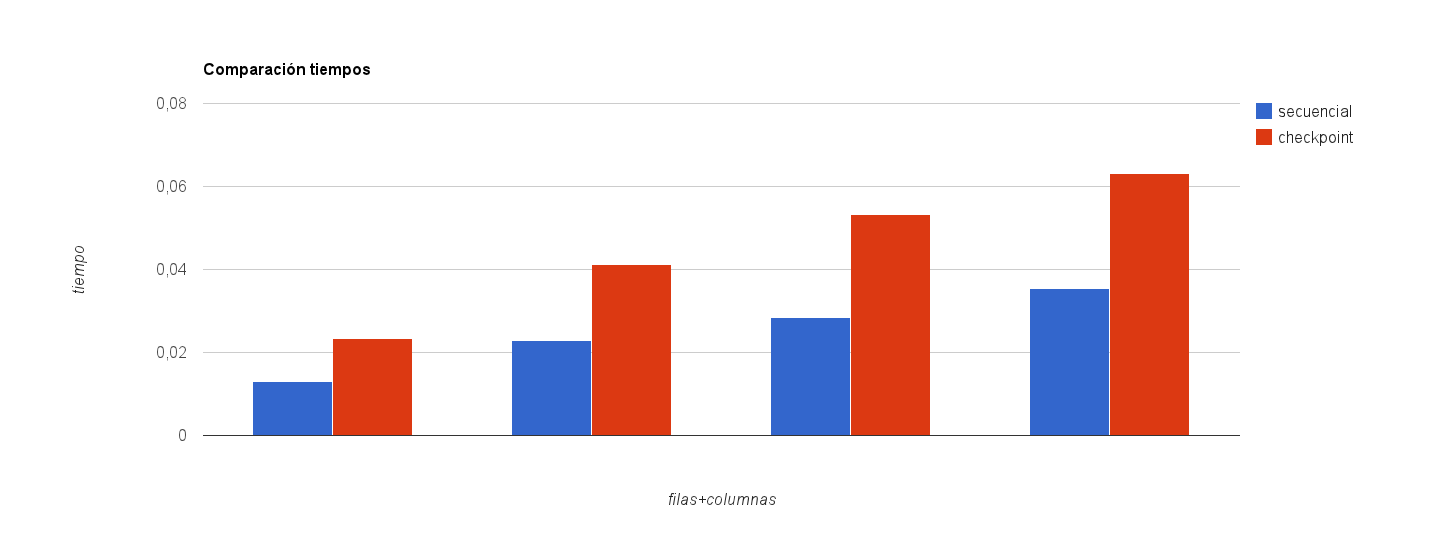
\includegraphics[width=1.2\textwidth]{res/comparacion_cp}
  \label{comp_cp}
  \caption{Comparación tiempos secuencial sin/con checksum sin fallo}
\end{figure}

Como vemos en la figura \ref{comp_cp}, al tener que almacenar la información de checksum empeoran los tiempos de ejecución.

Cuando hay un fallo y el programa tiene que cargar los datos a partir del checksum generado previamente, la carga realizada también tiene una repercusión sobre el tiempo de ejecución. Esto quiere decir que, si este coste es muy alto, en algunos casos será conveniente comenzar de cero en vez de reconfigurar el sistema.


En nuestro caso en particular, por la propia definición de la estructura de los ficheros \texttt{checkopoint} y \texttt{result}, sólo es necesaria la última fila de éstos para la reconfiguración, y los nombres de los ficheros de matrices para el checkpoint, que son las dos primeras filas; por lo que no se trata con grandes volúmenes de datos. Debería ser muy efectiva la reconfiguración y ser conveniente en la mayoría de los casos. En los casos que puede ser menos conveniente realizar la reconfiguración es en los que se han procesado pocos datos, por lo tanto es más eficiente calcular esos datos que reestaurar el sistema.


Esta teoría se prueba ejecutando el programa con matrices de $25*25$. Son matrices relativamente pequeñas y, en las pruebas realizadas, se ha ido parando el programa en diferentes puntos, calculando el tiempo de recuperación.


El coste de reconfigurar el sistema es del orden de $3 * 10^{-4}$.
En la implementación final del sistema, se decide guardar en el fichero de checkpoint, no sólo el último estado, si no todos los estados guardados. Para detectar fallos en caso de error. Con esta modificación, el fichero de checkpoint se hace más grande resultando en variaciones en el tiempo de recuperación, como se muestra en la figura \ref{tiempos_rec}

\begin{figure}[h!]
  %\centering
  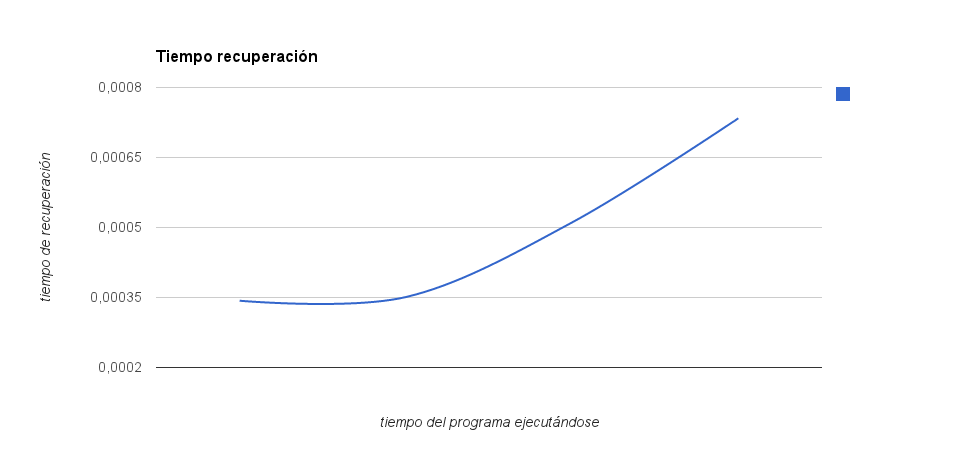
\includegraphics[width=1.2\textwidth]{res/tiempos_rec}
  \label{tiempos_rec}
  \caption{Tiempos de recuperación con fichero checksum con histórico}
\end{figure}
Pero lo importante es que, si guardamos los últimos estados del sistema (no todos), el rendimiento es bueno (tiempos de recuperación del orden de $3 * 10^{-4}$).

%\clearpage
%\section{Conclusiones}
%	\input{./conclusiones}

\end{document}
